\Chapter{Tervezés}

\section{UML}

\subsection{KeyHandler}

A KeyHandler osztály felel a kamera mozgatásáért, a játékmenet megállításért/elinditásáért, UI elemek használatáért, 
mint például az Inventory és Statistics oldal megnyitása/bezárása.

\subsection{Block}

Blockok néhány változóit tartalmazza.

\subsection{BlockManager}

Blockok típus definiálását, és a map beolvasást tartalmazza.

\subsection{GamePanel}

A játékmenet futását biztosítja.

\subsection{Camera}

Kamera kezdő helyzetét, lépés távját határozza meg.

\subsection{AssetSetter}

Az objektumok és ágensek elhelyezésért felelős.

\subsection{UI}

A gameScreenNumber változó által tárolt 3 fő képernyő megjelenítéséért felelős: Kezdő képernyő(title),
játékmenet(normal) és végsőképernyő(end).
Itt történnek a képernyőre való szöveg kiírások is.
Inventory és Statistics ablak megjelenítését is tartalmazza.

\subsection{Entity}

Röviden az ágensek útvonalválasztásáért felelős. 
Itt történik az életcsík megrajzolása is.
Tárolja az ágensek változóit.

\subsection{ItemDecider}

Entity osztálynak ad vissza igaz/hamis értékeket, amelyek befolyásolják az útvonalválasztást.

\subsection{Object}

Az objectek osztálya, object típusokat tartalmaz.

\subsection{Entity1}

Ágensek egyetlen típúsának alap értékeinek definiálására szolgál.

\subsection{EntityFaction1}

A faction 1-hez tartozó ágensek képeit tárolja, amelyeket láthatunk a szimulációban.

\subsection{EntityFaction0}

A faction 0-hez tartozó ágensek képeit tárolja, amelyeket láthatunk a szimulációban.


\begin{figure}[!ht]
	\centering
	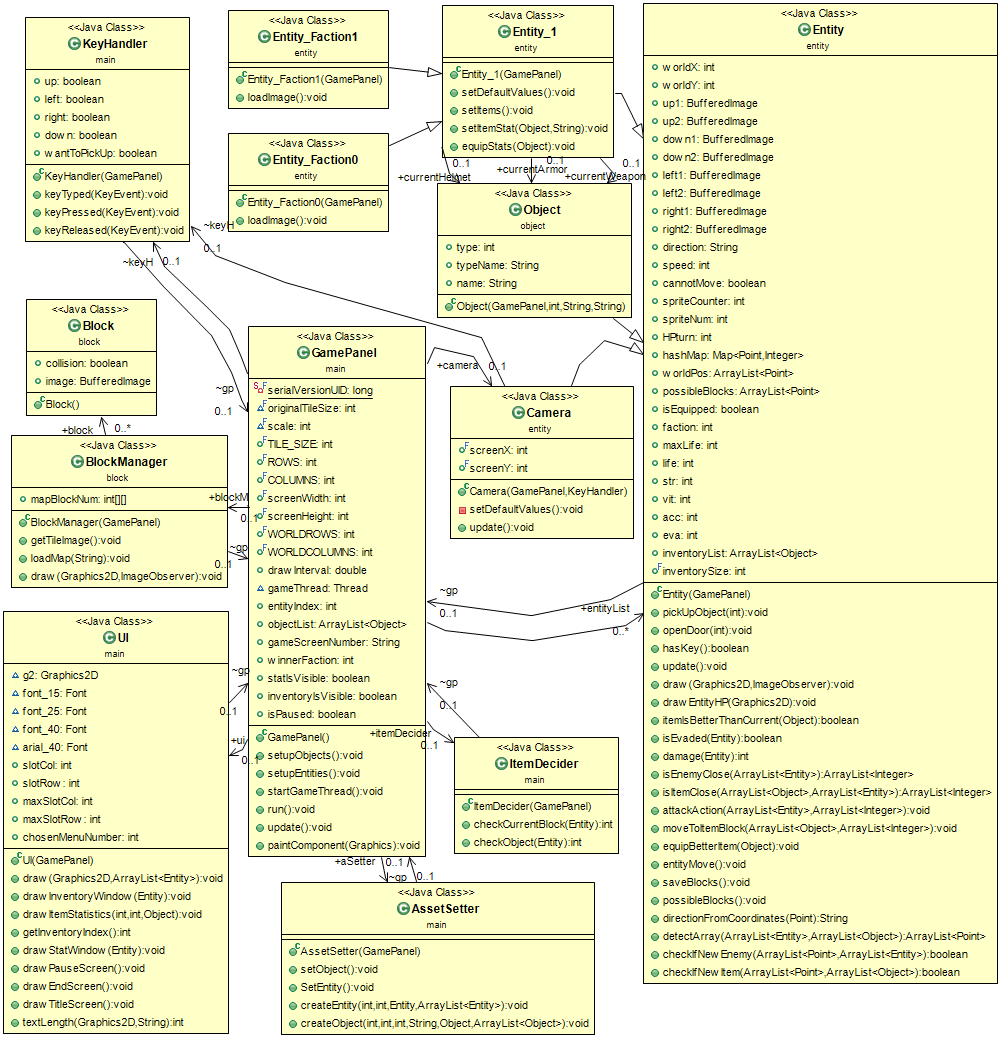
\includegraphics[scale=0.40]{images/UML.png}
	\caption{UML}
	\label{fig:UML}
\end{figure}